\section{Panoramica di possibili diverse architetture per Android Real-Time}
\subsection{Proposte ad alto livello}
\begin{figure}[h]
	\centering
	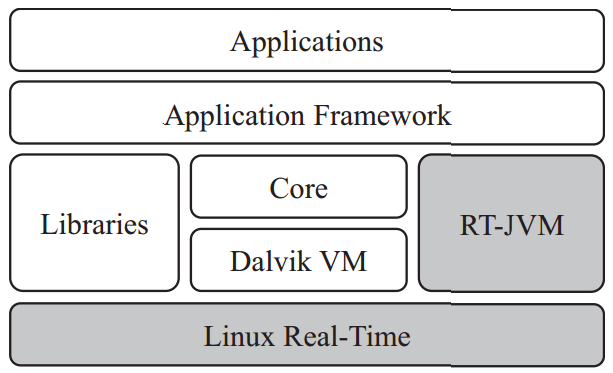
\includegraphics[width=0.7\linewidth]{androidPienoSupportoRT}
	\caption{Android Full real-time}
	\label{fig:androidpienosupportort}
\end{figure}
Una prima soluzione è mostrata in Figura~\ref{fig:androidpienosupportort} e considera la sostituzione di Linux con una versione real-time e l'aggiunta di una RT VM. Queste modifiche aggiungono prevedibilità e determinismo, ed è inoltre possibile aggiungere nuove politiche di scheduling attraverso le classi di scheduling e migliori strategie di gestione delle risorse. D'altra parte, però, tutti i driver utilizzati dal dispositivo devono essere implementati in un ottica real-time, e questo può portare a sforzi non necessari. La seconda modifica proposta riguarda l'aggiunta di una RT VM. Questa è considerata vantaggiosa, perché permette una gestione della memoria prevedibile. Inoltre, a seconda dell'algoritmo utilizzato, è anche possibile ottenere uno scheduling real-time, migliori meccanismi di sincronizzazione ed evitare l'inversione di priorità. Queste aggiunte sono assolutamente necessarie se si vuole ottenere una VM deterministica e prevedibile. Quest'ultima interagisce direttamente con il kernel per funzionalità come scheduling e gestione dei limiti di memoria. Non è necessario tenere il passo con le versioni di Android, perché è presente anche la DVM, ma è necessario implementare, la prima volta, una nuova Vm da zero e l'interprete Dalvik. Inoltre l'interazione di due VM può essere problematica, e può essere necessario pensare a nuovi algoritmi per ottimizzare lo scheduling.

\begin{figure}[h]
	\centering
	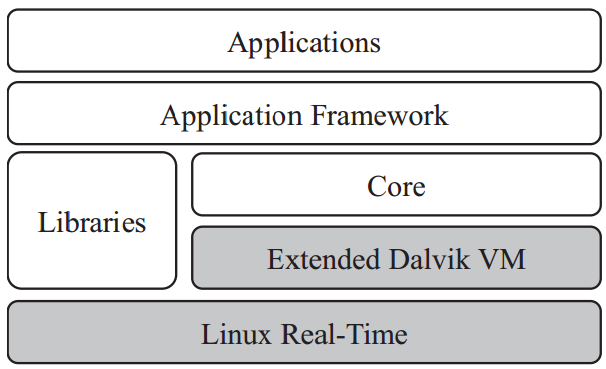
\includegraphics[width=0.7\linewidth]{androidEstesoRT}
	\caption{Android esteso con funzionalità real-time}
	\label{fig:androidestesort}
\end{figure}
La seconda soluzione è quella di sostituire Linux una versione real-time e di aggiungere funzionalità real-time a DVM (Figura~\ref{fig:androidestesort}). I vantaggi e gli svantaggi della sostituzione di Linux sono uguali a prima. Ora però la DVm viene estesa per supportare RTSJ. Questo permette di aggiungere alla DVm tutte le caratteristiche real-time previste dalla RTSJ, come GC real-time e gestione asincrona di eventi. In questo caso è però necessario stare al passo con i rilasci di nuove versioni della VM, per poter portare le modifiche a tutti i dispositivi Android.

\begin{figure}[h]
	\centering
	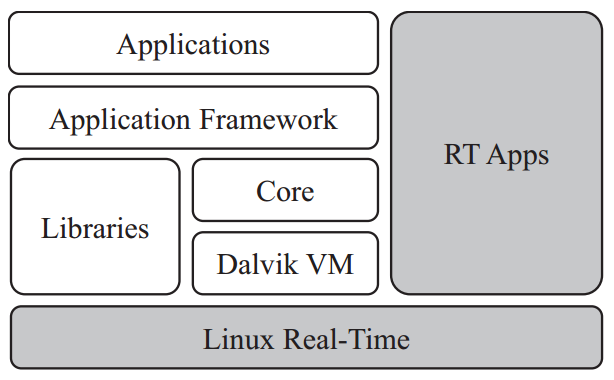
\includegraphics[width=0.7\linewidth]{rtandroidParziale}
	\caption{Android con support real-time parziale}
	\label{fig:rtandroidparziale}
\end{figure}
Il terzo approccio (Figura~\ref{fig:rtandroidparziale}) si basa ancora su Linux real-time e utilizza applicazioni real-time direttamente sopra il sistema operativo, utilizzando le librerie native. Questo è un vantaggio per quelle applicazioni che non necessitano della VM. Al contrario, però, le applicazioni che hanno bisogno della VM non possono avere supporto real-time.

\begin{figure}[h]
	\centering
	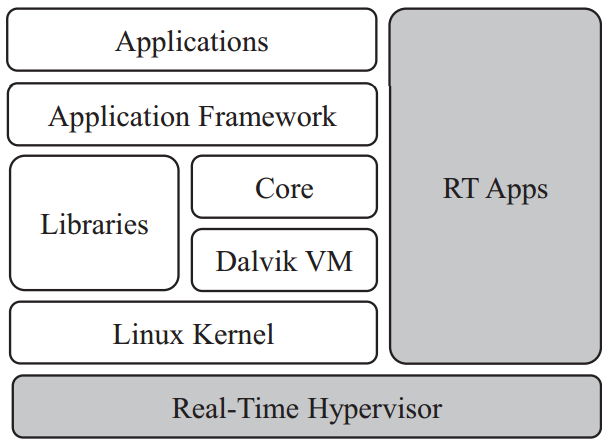
\includegraphics[width=0.7\linewidth]{androidConRTHypervisor}
	\caption{Android con real-time hypervisor}
	\label{fig:androidconrthypervisor}
\end{figure}
Il quarto approccio (Figura~\ref*{fig:androidconrthypervisor}) utilizza un real-time hypervisor in grado di eseguire parallelamente Android e applicazioni real-time. Questa soluzione è simile a quella utilizzata da alcuni sistemi operativi real-time, come RTLinux, e consiste nell'eseguire task real-time parallelamente (ma con priorità maggiore) a task del kernel. Lo svantaggio è che le applicazioni real-time godono delle sole funzionalità offerte dall'hypervisor, e quindi non possono utilizzare né i servizi della DVM né quelli di Linux. Inoltre, se un'applicazione real-time si blocca, l'intero sistema potrebbe bloccarsi.

\subsection{Liberare manualmente la memoria}
In \ref{sec:gcandroid} sono stati spiegate alcune criticità della GC in Android. Tuttavia, disabilitarla completamente non è una strada percorribile. Ogni processo ha la sua area di memoria e il GC viene invocato quando non c'è posto per soddisfare una richiesta di allocazione. Non liberare la memoria in questo contesto porterebbe sicuramente a comportamenti non prevedibili e distruttivi. Una soluzione più promettente potrebbe essere quella di liberare manualmente la memoria. In questo modo la probabilità che il GC sia invocato (e di conseguenza che l'applicazione venga bloccata) è minore. 

\begin{figure}[h]
	\centering
	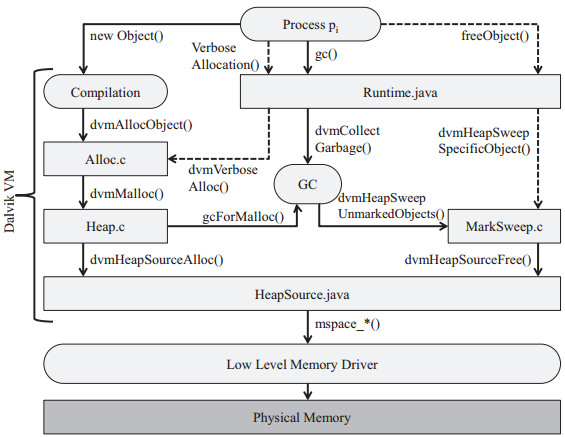
\includegraphics[width=0.7\linewidth]{../images/androidMemoryManagement}
	\caption{Gestione della memoria in Android}
	\label{fig:androidmemorymanagement}
\end{figure}

In Figura~\ref{fig:androidmemorymanagement} è mostrata la gestione della memoria in Android. Le transizioni rappresentano eventi di sistema, come chiamate di metodi, e mostrano i file sorgente coinvolti. I rettangoli arrotondati indicano entità astratte e componenti di sistema. Le linee tratteggiate rappresentano le estensioni proposte in questa soluzione. 

Durante la compilazione di un'applicazione Android, ogni istanziazione (\texttt{new}) viene tradotta in una chiamata a \texttt{dvmAllocObject()}. Questo metodo prende come argomento un riferimento alla classe richiesta. Tra le altre cose, questo riferimento contiene la dimensione dell'oggetto che si vuole creare. La dimensione viene passata a \texttt{dvmMalloc()}, che alloca la quantità di memoria desiderata. In generale, quest'ultima è responsabile della gestione degli errori, mentre l'allocazione vera e propria viene fatta da \texttt{dvmHeapSourceAlloc()}, che ritorna il risultato senza nessuna validazione. Se non ci sono errori, blocco viene poi convertito nell'oggetto e l'esecuzione continua. La chiamata può però fallire, ritornando un puntatore nullo e indicando la situazione della memoria. A questo punto \texttt{dvmMalloc()} prova a risolvere il problema avviando il GC,l dopodiché l'allocazione viene ripetuta o viene lanciata un'eccezione (\texttt{OutOfMemoryException}). Gli oggetti che non sono marcati dopo la passata del GC sono eliminabili. L'eliminazione viene fatta da \texttt{dvmHeapSweepUnmarkedObjects()}, che rilascia la memoria chiamando \texttt{dvmHeapSourceFree()} per ogni riferimento. Android offre anche la possibilità di richiedere esplicitamente la passata del GC, chiamando \texttt{Runtime.gc()} manualmente. Le chiamate esplicite al GC hanno gli stessi effetti negativi di quelle implicite. L'idea è quindi quella di pulire la memoria manualmente, oggetto per oggetto senza chiamare il GC. Sappiamo che \texttt{dvmHeapSourceFree()} offre la possibilità di eliminare un oggetto, dato il suo riferimento. Viene quindi aggiunto alla DVM un nuovo metodo, \texttt{dvmHeapSweepSpecificObject()}, che chiama \texttt{dvmHeapSourceFree()}. In più la classe \texttt{Runtime} viene estesa con il metodo \texttt{freeObject()}, per rendere disponibile la funzionalità per le applicazioni Android. \texttt{freeObject()} riceve come argomento un oggetto da rimuovere. Calcola il puntatore al blocco che contiene l'oggetto e lo passa a \texttt{dvmHeapSweepSpecificObject()}, che lo rimuove attraverso \texttt{dvmHeapSourceFree()}. Dopodiché la memoria è disponibile per un'altra allocazione. Uno svantaggio è che \texttt{freeObject()} può essere usato solo per quegli oggetti di cui lo sviluppatore è al corrente, ma la memoria può anche essere riempita di oggetti temporanei. Una soluzione è quella di aggiungere a \texttt{Runtime} anche il metodo \texttt{verboseAllocations()}, che permette di avere dei log su tutti gli oggetti che vengono allocati durante la vita di un processo. Questo log può poi essere usato per rendersi conto degli oggetti creati e liberare la memoria di conseguenza. 

\subsubsection{Valutazione}
In Figura~\ref{fig:valutazionegestionemanualememoria} viene mostrato un confronto fra la gestione della memoria manuale e con GC. Si nota che, raggiunti più o meno i 2900kB di memoria riferita, la DVM invoca il GC e l'applicazione viene, conseguentemente, bloccata. Al contrario, con la gestione manuale, il GC non viene mai invocato, perché la memoria riferita resta sempre sotto la soglia.
\begin{figure}[h]
	\centering
	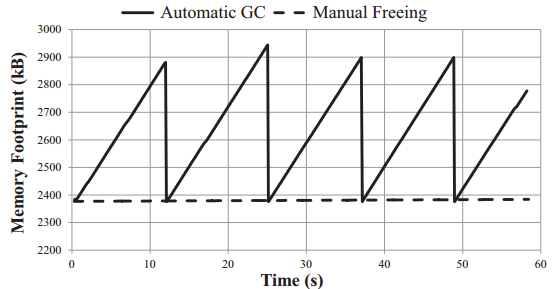
\includegraphics[width=0.7\linewidth]{valutazioneGestioneManualeMemoria}
	\caption{Valutazione della soluzione}
	\label{fig:valutazionegestionemanualememoria}
\end{figure}

Lo svantaggio e il limite evidente di questo approccio è che richiede che i programmatori gestiscano manualmente la memoria, proprio come in C o C++. Questo processo è estremamente difficoltoso, e può portare a molti leak e a gestioni scorrette. Sebbene prevenga l'invocazione del GC, gli errori introdotti dalla gestione manuale potrebbero portare l'applicazione ad un fallimento.

\subsection{Isolare una CPU per task real-time}
\begin{figure}[h]
	\centering
	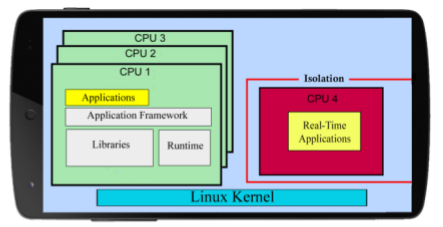
\includegraphics[width=0.7\linewidth]{cpuisolation}
	\caption{Isolare una CPU per eseguire applicazioni real-time}
	\label{fig:cpuisolation}
\end{figure}
Figura~\ref{fig:cpuisolation} mostra un altro possibile approccio. In questo caso una CPU viene isolata e riservata per l'esecuzione di applicazioni soft real-time. Nessun cambiamento al codice del kernel è richiesto (anche se la versione deve essere $>=$ di 2.6) e la soluzione è portabile su tutti i dispositivi.

Dalla versione 2.6 del kernel Linux, infatti, il flag \texttt{CONFIG\_PREEMPT} rende la maggior parte del kernel prerilasciabile. Alcuni dispositivi, infatti, possono generare interruzioni che verranno eseguite alla priorità più alta, portando a latenze anche molto elevate dei task real-time. Il flag, da solo, non è quindi abbastanza per fornire garanzie sui tempi di esecuzione. Tuttavia, sfruttando l'architettura multi-core della maggior parte dei dispositivi Android, è possibile isolare una CPU da scheduler e interruzioni ed eseguire tutti i processi con requisiti real-time su di essa. 

\subsubsection{Isolare la CPU}

\paragraph{Isolcpus} \mbox{} \\
Dalla versione 2.6.9, Linux include un parametro di boot, \textit{isolcpus}, che permette di stabilire una lista di processori isolati. Questi non saranno mai utilizzati dallo scheduler, eccetto che per eseguire thread del kernel e interruzioni. Un task può essere eseguito su una CPU isolata utilizzando la chiamata di sistema \texttt{sched\_affinity} o il comando \texttt{taskset}.

Isolcpus è un parametro di boot, e quindi non può essere cambiato dopo l'avvio. Settare questo parametro in Android è complicato, perché molti produttori utilizzano dei bootloader proprietari. È dunque necessario fare il flash dell'immagine di ANdroid modificata per utilizzare questo flag.

\paragraph{Cpuset} \mbox{} \\
Mentre Android esegue un'applicazione, i servizi in background e gli altri programmi possono rallentare l'esecuzione. Per risolvere questo problema viene utilizzata una funzionalità del kernel chiamata \textit{cgroups} (control groups) che limita l'utilizzo di CPU per un insieme di processi.

Ci sono due meccanismi usati da Android per influenzare lo scheduling: il \textit{nice} level e i cgroups. Il nice level influenza lo scheduling fair, nel senso che maggiore è il nice level meno frequentemente il processo verrà eseguito. Apparentemente questo potrebbe assicurare che l'applicazione in foreground non sia influenzata da chi è in background, ma, in pratica, non basta, perché molte applicazioni e servizi potranno essere in background e avere services in attesa di esecuzione. Quindi Android usa anche i cgroups per distinguere tra foreground e background, e sono attivi per default nel kernel. Inoltre, esiste una funzionalità chiamata cpuset che assegna singole CPU agli cgroups. Lo scopo è quello di porre restrizioni sulle risorse utilizzabili da un processo. Android, però, non l'ha abilitato per default, e deve essere fatto a mano. I cpusets sono rappresentati come directory in un file system pseudogerarchico, dove la top directory (\texttt{/dev/cpuset}) rappresenta l'intero sistema e ogni cpuset che è figlio di un altro cpuset contiene un sottoinsieme delle CPU e dei nodi di memoria utilizzabili dal padre. 

Un processo esegue solo nelle CPU corrispondenti al suo cpuset. Di conseguenza è possibile creare un cpuset per i task real-time, ed usare tutte le altre CPu per gli altri. L'idea è mostrata in Figura~\ref{fig:cpuset}.
\begin{figure}[h]
	\centering
	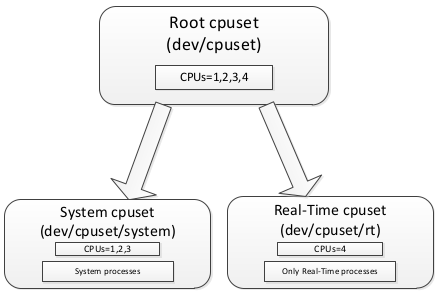
\includegraphics[width=0.7\linewidth]{cpuset}
	\caption{Due cpusets per isolare task real-time}
	\label{fig:cpuset}
\end{figure}

\paragraph{Vincitore} \mbox{} \\
Entrambi i meccanismi possono essere usati per isolare un core in un'architettura multi-core. Ci sono però degli svantaggi nell'uso di Isolcpus. Primo, può essere avviato solo durante il boot, spesso dovendo fare una rebiuld e il flash dell'immagine. cpuset, al contrario, può essere cambiato a run-time. Secondo, isolcpus permette allo scheduler di assegnare task alle CPU isolate, e non è possibile impedire ad un'applicazione di chiamare \texttt{sched\_affinity} sulla CPU riservata. In cpuset, invece, l'allocazione del processo deve essere fatta scrivendo esplicitamente il PID in un file usato per la configurazione. Per modificarlo è necessario avere i privilegi di root.

Tuttavia, nessuno dei due approcci può controllare dove verranno eseguiti i processi del kernel, perché questi non possono essere assegnati in una specifica CPU.

\paragraph{SMP IRQ Affinity} \mbox{} \\
I componenti hardware inviano delle interruzioni a CPU specifiche per chiedere attenzione. Queste interruzioni non sono direttamente evitabili isolando le CPU. A partire dalla versione 2.4 del kernel, Linux ha introdotto la possibilità di assegnare alcune richieste di interruzione (IRQ) a specifiche CPU. Questa possibilità è nota con il nome di \textit{SMP IRQ Affinity}, e permette di controllare quali core gestiranno quali interruzioni. Per ogni IRQ c'è una directory in \texttt{/proc/irq}, che contiene il file \texttt{smp\_affinity}, dove è possibile cambiare l'affinità interruzione-CPU. Di conseguenza si può lasciare un core isolato, e far eseguire le interruzioni sulle altre CPU, anche se non tutte sono modificabili (ad esempio le \textit{inter-processor interrupts} non lo sono).

\paragraph{Utilizzo di meccanismi di isolamento delle CPU per lo scheduling real-time} \mbox{} \\
Il meccanismo di isolamento descritto sopra permette di eseguire task in un core isolato, riducendo quindi significativamente l'interferenza subita. In aggiunta a questo serve uno scheduler real-time. Come già detto, due politiche real-time sono fornite da linux (\texttt{SCHED\_RR} e \texttt{SCHED\_FIFO}). La politica \texttt{SCHED\_DEADLINE}, che implementa EDF, è stata aggiunta nella versione 3.14, ma le versioni del kernel per Android sono ancora precedenti a quella release.

La politica più usata è dunque \texttt{SCHED\_FIFO}, che implementa un algoritmo a fixed-priority con comportamento FIFO quando la priorità è la stessa. Un task continua ad eseguire finché non si sospende volontariamente, non si blocca o non viene prerilasciato da un task a più alta priorità. \texttt{SCHED\_RR} è simile, ma se la priorità è la stessa a tutti i task viene assegnato uno slice temporale per eseguire (in \texttt{SCHED\_FIFO} un task non prerilascia un altro task con la stessa priorità).

\paragraph{Aggiustamenti generali} \mbox{} \\
Alcuni accorgimenti sono necessari:
\begin{itemize}
	\item aggiustare la frequenza della CPU per evitare variazioni dei tempi di risposta. Questo vale solo per le CPU dedicate ai task real-time;
	\item molti dispositivi hanno demoni utilizzati per risparmiare energia, e spengono le CPU non utilizzate. La CPU dei real-time deve sempre essere attiva, quindi questi demoni devono essere bloccati e le CPU isolate devono essere sempre attive;
	\item l'opzione \texttt{CONFIG\_CPUSETS} deve essere abilitata per usare cpuset. Di default non è attiva;
	\item è necessario anche attivare il flag \texttt{CONFIG\_PREEMPT}.
\end{itemize}

\subsubsection{Valutazione}
I test eseguiti confermano che la migliore configurazione è quella con isolamento utilizzando cpuset, con politica di scheduling \texttt{SCHED\_FIFO} e SMP IRQ Affinity. Utilizzando cpuset, infatti, c'è la certezza che nessun altro task venga assegnato alla CPU isolate, riducendo quindi l'interferenza. Inoltre, in 1 secondo di run-time, il jitter con l'isolamento è di appena 46 $\mu~s$, mentre senza isolamento arriva anche a 1.5s. Il tempo di risposta è quindi notevolmente migliore.

Sebbene questa soluzione sia molto versatile, perché non richiede pesanti modifiche al kernel, non supporta l'interazione tra applicazioni real-time, e queste ultime non possono essere scritte in Java. Infatti, dato che non viene fatta nessuna modifica alla VM, questa continuerà a comportarsi in modo non real-time.